\bghdr{images/fond-win}

%\begin{center}
%
\includegraphics{images/logo_Windows}
%\end{center}


\subsection{Configuration sous Microsoft Windows}

Cette section décrit comment configurer un ordinateur tournant sous Windows XP ou sous Windows Vista. Si tu possèdes une autre version de Windows,
nous t'invitons à regarder directement la section sur les licences MSDNAA en page \pageref{msdnaa}\dots ou alors à te débrouiller ! ;-)

\subsubsection{Configuration IP}

\begin{itemize}

\item \textbf{Sous Windows XP :} va dans le \menu{Menu Démarrer}, \menu{Panneau de configuration} et double-clique sur \menu{Connexions réseau} puis sur \menu{Connexion au réseau local}. Clique enfin sur \menu{Propriétés}.

\item \textbf{Sous Windows Vista :} va dans le \menu{Menu Démarrer}, \menu{Panneau de configuration}, \menu{Réseau et Internet}, \menu{Centre réseau et partage}. Là, dans le menu à gauche, clique sur \menu{Gérer les connexions réseau}, puis clique droit sur \menu{Connexion au réseau local} et enfin  \menu{Propriétés}~\footnote{\`A ce stade, ainsi qu'à plusieurs autres étapes de ce tutoriel, Windows Vista doit normalement t'afficher un message te demandant de confirmer l'action que tu viens d'effectuer. Donc tu confirmes, et cela à chaque fois !}.

\end{itemize}



%\flimage{images/win_connexion_icone}{0.15}{l} Va dans le \menu{Menu
%Démarrer}, \menu{Panneau de configuration} et double-clique sur
%\menu{Connexions réseau} puis sur \menu{Connexion au réseau local}.
%Clique enfin sur \menu{Propriétés}.\\

%Dans cette fenêtre, coche les trois cases \menu{Client pour les
%réseaux Microsoft}, \menu{Partage de fichiers} et \menu{Protocole
%Internet (TCP/IP)}:

\imagepos{images/win_config_connexion2}{0.5}{Configurer la connexion au réseau local}{!h}



%\imageref{images/win_config_ip}{0.5}{Configuration IP --- Propriétés de protocole Internet (TCP/IP)}{!ht}{config:win:IP1}
%%%%\imageref{images/win_config_ip2}{0.71}{Configuration de la connexion
%au réseau local et propriétés du TCP/IP}{!ht}{config:win:IP1}

Sélectionne ensuite la ligne \menu{Protocole Internet Version 4 (TCP/IPv4)}~\footnote{\menu{Protocole Internet (TCP/IP)} pour certaines versions de Windows XP.},
puis clique sur le bouton \menu{Propriétés} qui vient de se
dégriser. Tu tombes alors sur l'écran de configuration de ta
connexion vers l'extérieur.

\noindent
  \begin{figure*}[!h]
    \begin{center}  
      \subfloat[Configuration IP --- Propriétés de protocole Internet (TCP/IP)]{ 
      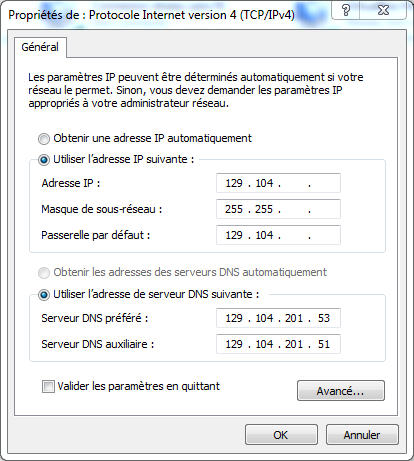
\includegraphics[width=0.48\textwidth]{images/win_config_ip} \label{config:win:IP1}}
      \hspace{\stretch{1}}
      \subfloat[Configuration DNS]{ 
 		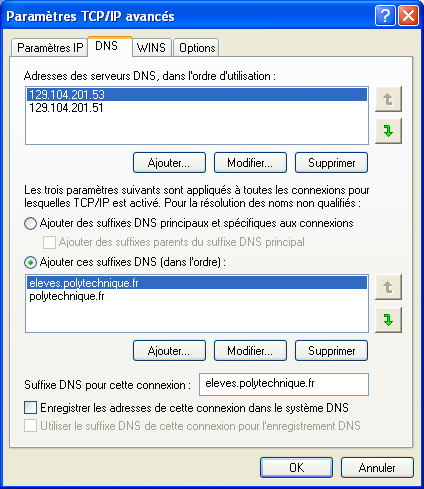
\includegraphics[width=0.48 \textwidth]{images/win_config_dns2} \label{config:win:IP2}}
         	 \caption{Configuration réseau}
    \end{center}
  \end{figure*}



%% \newpage
Coche alors les cases \menu{Utiliser l'adresse IP suivante} et \menu{Utiliser l'adresse de serveur DNS suivante} et remplis les cinq champs d'adresse IP. Tu trouveras toutes les valeurs d'adresse IP nécessaires pour la configuration en page~\pageref{tableau:mon_IP} ; aide-toi de la capture d'écran~\ref{config:win:IP1} pour les placer. Si une partie d'adresse IP est blanche sur cette capture, c'est qu'elle t'est personnelle et que tu dois la calculer !
Clique, ensuite sur le bouton \menu{Avancé}, puis sur l'onglet
\menu{DNS} en haut.
Il n'y a plus qu'à remplir les différents champs comme sur la
capture d'écran suivante, avec le bouton \menu{Ajouter} et les
flèches pour réordonner les éléments.


%\subsubsection{Le domaine Windows}

%\paragraph{Qu'est ce que c'est ?}
%Le domaine Windows est un système d'automatisation de la
%configuration de plusieurs ordinateurs sous Windows situés sur le
%même réseau. En fait, c'est un outil d'administration, con\c{c}u par
%exemple pour des entreprises o\`u un service informatique doit gérer
%de nombreuses machines; il permet d'appliquer des modifications de
%configuration à toutes les machines du domaine directement depuis un
%serveur. Le BR possède un serveur dédié au domaine Windows,
%\server{enez}.

%Le domaine met à jour automatiquement Windows et l'antivirus à partir d'\server{enez} (très rapide car tu n'as pas besoin de récupérer des fichiers
%en dehors de l'école!). Il configure le \emph{firewall} (pare-feu: système de protection contre les éventuelles attaques par le réseau) Windows, mais
%il est toujours possible de le désactiver si tu préfères un autre \emph{firewall}. En bref, il permet de simplifier à l'extrême %la mise à jour
%continuelle de l'ordinateur.%


%\paragraph{Alors, domaine ou pas domaine ?} Soit tu choisis de te
%mettre sur le domaine Windows, et tu vas alors au paragraphe
%\guillemotleft~Inscription sur le domaine Windows~\guillemotright.%

%% \newpage
%\textbf{Avantages :}
%\begin{itemize}
%\item Windows est mis à jour automatiquement ; tu as toujours les
%dernières corrections de sécurité et un pare-feu correctement
%configuré. Donc tu es mieux protégé contre les intrusions.
%\item Surtout, tu n'as plus à t'en occuper, presque tout est automatique.
%\end{itemize}%

%\textbf{Inconvénients :}
%\begin{itemize}
%  \item Tu délègues une partie des droits d'administration de ta machine au BR
%        (tout ce qui concerne la sécurité du réseau en particulier).
%        Cependant, si tu ne sais pas le faire, c'est plut\^ot un avantage
%        de laisser le BR s'en occuper à ta place.
%  \item Cela ne marche qu'avec Windows 2000, Windows XP Pro ou Windows Vista Business.
%        On te rappelle que tu peux facilement, gratuitement et légalement passer à
%        Windows XP Pro ou bien à Windows Vista Business (section sur les licences
%        MSDNAA en page \pageref{msdnaa}).
%\end{itemize}

%Bien s\^{u}r, tu peux sortir du domaine à tout instant, et effectuer manuellement les réglages nécessaires à la sécurité de ton ordinateur.

%Soit tu choisis de configurer toi-même ton ordinateur, et tu peux passer
%directement à la section \guillemotleft Installation de l'antivirus
%\guillemotright. Tu trouveras les informations nécessaires à la configuration
%manuelle du pare-feu et du proxy pour \app{Windows Update} en annexe à la
%fin de cette section, en page \pageref{horsdomaine}.

%\textbf{Avantage :} Tu es le seul à t'occuper de la gestion de ton ordinateur.

%\textbf{Inconvénient :} Tu es le seul à t'occuper de la gestion de ton ordinateur. ;-)
%S'il devient un foyer pour virus, sache que nous avons les moyens de l'isoler
%pour éviter toute propagation.

%\begin{center}
%  \fbox{
%    \begin{minipage}{.7\textwidth}
%      \begin{center}
%Le BR te conseille \emph{très fortement} de te mettre sur le domaine
%et de choisir l'installation simplifiée !
%      \end{center}
%    \end{minipage}
%  }
%\end{center}


%\paragraph{Inscription sur le domaine Windows}

%On te rappelle que tu ne peux t'inscrire sur le domaine que si tu utilise
%Windows 2000, Windows XP Pro ou Windows Vista. Si tu possède Windows XP
%Familial, Windows Vista Home ou encore une version antérieure de Windows,
%tu dois effectuer toi-même tes réglages de pare-feu et de proxy
%\app{Windows Update}. Réfère-toi pour cela à l'annexe ad hoc à la fin de
%cette section, en page \pageref{horsdomaine}.

%La procédure d'inscription est la suivante :
%\begin{itemize}

%\item \textbf{Sous Windows XP :} Clique sur le \menu{Menu Démarrer} puis fais un clic-droit sur
%\menu{Poste de travail} et choisis \menu{Propriétés}. Ensuite, sélectionne l'onglet \menu{Nom de l'ordinateur} et clique le bouton \menu{Modifier}.

%\item \textbf{Sous Windows Vista :} Clique sur \menu{Menu Démarrer}, puis fais un clic-droit sur \menu{Ordinateur}, \menu{Propriétés}. Là sélectionne \menu{Paramètres système avancés}, onglet \menu{Nom de l'ordinateur}, puis clique sur le bouton \menu{Modifier}.

%\end{itemize}

%Dans la case \menu{Nom de l'ordinateur}, rentre ton pseudo, puis coche la case \menu{domaine} et
%rentre \urllink{windows.eleves.polytechnique.fr}. Note bien que l'inscription au domaine te sera
%refusée par le serveur si quelqu'un d'autre utilise déjà le même nom d'ordinateur que toi. Par
%conséquent, essaie d'opter pour un pseudo qui t'identifie de fa\c{c}on claire et unique, par exemple
%\cmd{NOM\_PRENOM} \footnote{Les Jean Dupont et les Julien Thomas sont priés de trouver autre chose
%;-)}.

%\imagepos{images/win_config_domaine}{0.5}{S'inscrire sur le domaine windows}{!ht}

%\begin{center}
%\begin{tabular}{ll}
% \parbox{.45\textwidth}{
%  et si tu es rouje 2006 :
%  \begin{description}
%    \item[Nom] rouje06
%    \item[Mot de passe] rouje.2006
%  \end{description}
 % }
% & \parbox{.45\textwidth}{
%  Si tu es j\^one 2007, tu rentres :
%  \begin{description}
%    \item[Nom] jone07
%    \item[Mot de passe] jone.2007
%  \end{description}
%  }
%\\
%\end{tabular}
%\end{center}

%\emph{Attention, ces identifiants servent juste à t'inscrire sur le
%domaine. Pour utiliser ton ordinateur, tu devras rentrer au
%démarrage les mêmes nom d'utilisateur et mot de passe que tu avais
%avant d'être sur le domaine !}
%
%
%
%%\paragraph{Installation personnalisée} --- configuration manuelle

%\subparagraph{Configuration antivirus} Le BR, concerné par la
%sécurité du réseau, te propose un antivirus pour lequel tu n'auras
%pas à payer la license pour obtenir les mises à jour. Bien s�r,
%libre à toi d'utiliser ton anti-virus personnel ; cependant il sera
%à ta charge de le mettre à jour très réguliérement. Pour cela
%utilise comme proxy : \urllink{http://kuzh} sur le port 8080.

%\emph{Installation de l'anti-virus du BR}\ : Commence par
%désinstaller tous les antivirus ou firewalls que tu pourrais avoir
%comme expliqué dans le paragraphe \guillemotleft~Installation simplifiée
%--- configuration automatique~\guillemotright .

%Puis ouvre ton explorateur Windows et tape :
%\urllink{$\backslash\backslash$enez$\backslash$antivirus}
%et double-clique sur le fichier \file{Symantec.exe}.

%Ce package contient le paramétrage de la mise à jour automatique de
%Windows sur le serveur de l'école. Attends la fin de l'installation
%et c'est fini ! Maintenant, tu n'as plus à toucher à l'antivirus,
%normalement il sera mis à jour automatiquement.

%\subparagraph{Configuration firewall}

%Si tu as Windows XP avec le SP2 installé, tu as un firewall
%automatiquement activé et facile d'utilisation. En effet, à chaque
%fois qu'un programme tentera d'aller pour la première fois sur
%Internet, il te demandera si tu veux le laisser faire ou non, comme
%dans la capture~\ref{config:win:firewall}.

%\imageref{images/win_firewall}{0.8}{Un programmme --- ici GuildFTP
%--- demande à accéder au réseau}{!ht}{config:win:firewall}

%Le firewall commercial \app{ZoneAlarm}, indépendant de Windows,
%fonctionne sur le même principe. Tu peux le trouver sur \xshare.

%Si tu préfères utiliser le firewall intégré à Windows XP (sans le
%SP2) ou à Windows Server 2003, il te faudra le configurer en détail.
%Va dans le \menu{Menu Démarrer}, \menu{Paramètres} et clique sur
%\menu{Connexions Réseau}. Choisis la connexion qui est utilisée par
%ton ordinateur (souvent il n'y en a qu'une, ou alors une seule est
%activée) et double-clique dessus. Clique sur \menu{Propriétés} en
%bas à gauche, puis sur l'onglet \menu{Avancé} et rentre dans le menu
%de \menu{Paramètres} du \menu{Pare-feu Windows}. Il te faudra alors
%ajouter manuellement tous les ports que tu veux ouvrir sur
%l'extérieur. Pour cela, clique sur \menu{Ajouter}, et remplis la
%bo�te de dialogue en t'aidant de la capture
%d'écran~\ref{config:win:ouvrir_port}; mets le numéro du port que tu
%veux ouvrir, par exemple 5050, 5053 et 5055 en TCP pour \app{qRezix}
%et 21 en TCP pour ton FTP.

%\imageref{images/win_config_firewall}{0.7}{Ouvrir un port dans le firewall %Windows}{!ht}{config:win:ouvrir_port}

%Comme tu peux le constater, il est beaucoup plus pratique d'aller
%sur le domaine et de laisser le SP2 faire le gros du boulot à ta
%place :-).


\subsubsection{Installation de l'antivirus}
\label{antivirus} Le BR, préoccupé par la sécurité du réseau, te propose un antivirus~\footnote{En
l'occurence, l'antivirus utilisé est \app{Symantec Antivirus 10.2}.} pour lequel tu n'auras pas à
payer de licence pour obtenir les mises à jour. Bien s\^{u}r, libre à toi d'utiliser ton antivirus
personnel ; cependant il sera à ta charge de le mettre à jour très régulièrement. Pour cela,
utilise comme serveur mandataire (\emph{proxy}) : \urllink{kuzh.polytechnique.fr} sur le port 8080 (il y a aussi des fois o\`u il 
faut rentrer \urllink{http://kuzh.polytechnique.fr}).

%Version pour vista à taper
Tout d'abord, \emph{désinstalle tous les antivirus que tu pourrais
avoir !} Dans le \menu{Menu Démarrer}, va dans \menu{Panneau de
Configuration}, \menu{Ajout/Suppression de Programmes} et
désinstalle si tu l'as \app{Symantec Antivirus}, \app{McAfee Antivirus}, \app{Norton
Antivirus}, ou tout autre antivirus.

Il s'agit ensuite de télécharger la bonne version de l'antivirus :
\begin{itemize}

\item Si tu as Windows Vista\dots
\begin{itemize}
\item en version 32 bits : \urllink{ftp://enez/antivirus/Win32\_Vista.zip}.
\item en version 64 bits : \urllink{ftp://enez/antivirus/Win64\_Vista.zip}.
\end{itemize}

\item Si tu as Windows XP ou une autre version de Windows\dots
\begin{itemize}
\item en version 32 bits : \urllink{ftp://enez/antivirus/Win32\_PasVista.zip}.
\item en version 64 bits : \urllink{ftp://enez/antivirus/Win64\_PasVista.zip}.
\end{itemize}
\end{itemize}

Si tu ne sais pas si ton Windows est 64 ou 32 bits, le plus problable est qu'il
soit 32 bits, donc tu peux commencer à essayer avec cette version.

Une fois le fichier adéquat téléchargé, ouvre l'archive compressée \file{Win\?\?\_*.zip}, décompresse \emph{tous les fichiers} dans un dossier et exécute le fichier \file{setup.exe} qui vient d'apparaître dans ce dossier. \`A partir de là, tu n'as plus qu'à suivre les instructions du
programme d'installation. Tu n'auras alors plus à toucher à l'antivirus, celui-ci sera mis à jour automatiquement.

\subsubsection{Configuration \emph{web} (serveur mandataire)}

\imageref{images/win_config_proxy}{0.5}{Configuration du serveur mandataire (\emph{proxy})}{!ht}{config:win:proxy}

Même si tu n'utilises pas \app{Internet Explorer} comme client \emph{web}, Windows et d'autres programmes
utilisent ses paramètres, notamment \app{Windows Update}. Donc lance \app{Internet Explorer} et va
dans le menu \menu{Outils}, \menu{Options Internet}, puis sur l'onglet \menu{Connexions} de la
nouvelle fenêtre et enfin sur \menu{Paramètres réseau} dans le bas de la fenêtre. Là, coche
uniquement la case \menu{Utiliser un script de configuration automatique}, puis remplis le champ
\menu{Adresse} avec \urllink{http://frankiz/proxy.pac}. Tu dois alors avoir quelque chose qui
ressemble à la capture d'écran~\ref{config:win:proxy}.

Une fois que tu as fait \c{c}a, tu n'as plus forcément besoin d'\app{Internet Explorer} tu peux donc utiliser un autre navigateur, comme \app{Mozilla
Firefox}, disponible sur \xshare, qui est plus sécurisé. Mais ce n'est pas une garantie ultime --- tu es le premier garant de la sécurité de ton
ordinateur, en n'ouvrant pas tous les fichiers qui te passent sous la main
--- mais tu seras sensiblement plus en sécurité.



Si tu utilises \app{Mozilla Firefox}, il faut que tu fasses, en plus, le même réglage de serveur mandataire pour
ce navigateur. Pour ce faire, lance \app{Mozilla Firefox}, et va dans le menu \menu{Outils},
\menu{Options...}. Là, sélectionne la rubrique \menu{Avancé}, onglet \menu{Réseau}, et clique sur
\menu{Paramètres}. La case à cocher est alors \menu{Adresse de configuration automatique du proxy},
et l'adresse à indiquer est la même que précédemment : \urllink{http://frankiz/proxy.pac}.

%
% Pour le RTFIBRp11 pour un saut de page si nécéssaire ce qui n'était pas le cas en 2008

%\noindent\rule{.4\textwidth}{.4pt}

%\vfill %\pagebreak

\subsubsection{Configuration \emph{mail}}

\footnote{Pour des raisons historiques, cette page porte le numéro 31. L'explication se trouve en page 11.} La DSI met à ta disposition une bo\^{i}te aux lettres électronique sur
le serveur \server{poly} ; cette section t'explique comment
configurer \app{Outlook Express} et \app{Windows Mail} pour y avoir accès. Tu peux bien
s\^{u}r utiliser \app{Thunderbird} si tu préfères, les données à rentrer
pour la configuration sont les mêmes ; quelques détails sont donnés
dans le WikiX sur \fkz. De plus, tu trouveras des explications plus
détaillées dans le manuel rédigé par la DSI.
La procédure suivante fonctionne aussi avec \app{Windows Mail}.
Lance \app{Outlook Express} et va dans le menu \menu{Outils},
\menu{Comptes\ldots}. Clique sur le bouton \menu{Ajouter\ldots} en
haut à droite, puis sur \menu{Courrier\ldots}, pour \app{Windows Mail} c'est sur compte de messagerie qu'il faut cliquer, avant de cliquer sur suivant.

%\setcounter{page}{31}


Remplis les écrans de configuration suivants avec ces données :
\begin{description}
  \item[Nom complet] ton nom (\guillemotleft~Martin Durand~\guillemotright , par exemple)
  \item[Adresse de messagerie] de la forme \mail{prenom.nom@polytechnique.edu}
  \item[Type de serveur de messagerie pour le courrier entrant] \menu{POP3}
  \item[Serveur de messagerie pour le courrier entrant] \server{poly.polytechnique.fr}
  \item[Serveur de messagerie pour le courrier sortant] \server{poly.polytechnique.fr}
  \item[Nom du compte] ton \emph{login} \server{poly} (les huit premières lettres de ton nom en général; si tu ne t'en souviens pas ne t'en fais pas on devrait te le redonner en cours d'informatique lors de ton premier TD. Si tu es vraiment pressé va voir le bureau \emph{login} de la DSI.)
  \item[Mot de passe] ton mot de passe \server{poly} ;
       vérifie bien que la case \menu{Mémoriser le mot de passe} est cochée.
\end{description}

Voilà, clique sur \menu{Continuer}, \menu{Terminer}.

Tu te retrouves alors sur la fenêtre \menu{Comptes Internet}. Va sur
l'onglet \menu{Courrier}, clique sur le compte que tu viens de créer
puis sur \menu{Propriétés}. Clique sur l'onglet \menu{Avancé} et
configure comme sur la capture~\ref{config:win:mail} ; en
particulier, coche la seconde case \menu{Ce serveur nécessite une
connexion sécurisée (SSL)}.

Comme \c{c}a, tu peux désormais recevoir des \emph{mails} avec une liaison
sécurisée vers \server{poly} pour que personne ne puisse les
intercepter.


\imageref{images/win_config_mail_avance}{0.5}{Configuration avancée
des serveurs \emph{mail}}{!h}{config:win:mail}

\subsubsection{Configuration \emph{newsgroups}}

Reporte-toi a la page~\pageref{newsgroups} pour la description et des détails de fonctionnement des \emph{newsgroups} à l'X.

Comme pour les \emph{mails}, nous décrivons la configuration de \app{Outlook Express} mais elle est sensiblement équivalente pour \app{Thunderbird}. Lance
\app{Outlook Express} et va dans le menu \menu{Outils}, \menu{Comptes\ldots}. Clique sur le bouton \menu{Ajouter\ldots} en haut à droite,
\menu{News\ldots}. Remplis les écrans de configuration suivants avec ces données :
\begin{description}
  \item[Nom complet] ton nom !
  \item[Adresse de messagerie] de la forme \mail{prenom.nom@polytechnique.edu}
  \item[Serveur de news (NNTP)] \fkz ; vérifie à ce moment que la case
       \menu{Connexion à mon serveur de news requise} n'est pas cochée.
\end{description}
Voilà, clique sur \menu{Continuer}, \menu{Terminer}; tu es abonné
au serveur \emph{news} des élèves.

Quand tu fermeras la fenêtre `Comptes Internet', il va te demander à
quels \emph{newsgroups} tu veux t'abonner, tu n'auras qu'à sélectionner
ceux qui t'intéressent. Reporte-toi à la page \pageref{newsgroups}
pour plus d'infos sur les newsgroups auxquels t'abonner !

Si tu veux t'inscrire à d'autres serveurs \emph{news}, refais cette
procédure en rentrant le nom du serveur qui t'intéresse à la place
de \fkz, par exemple \server{polynews.polytechnique.fr} pour accéder aux news externes.
%\setcounter{page}{12}

\subsubsection{Configuration FTP}

\paragraph{Client FTP}
Le BR te conseille \app{FileZilla} ou \app{SmartFTP}. Pour installer l'un des deux, télécharge-le sur \xshare et double-clique sur l'installeur.
Tu pourras dès la fin de l'installation aller sur tous les FTP du réseau
facilement et rapidement.

\paragraph{Serveur FTP}
Tu verras rapidement que tout le monde à l'X possède un serveur FTP
afin de partager les différents projets, les films du JTX, ses
photos, etc. Il est donc quasiment indispensable que tu en installes
un.

Parmi les plus simples on trouve \app{FileZilla Server} et \app{GuildFTP}, qui sont libres de surcro\^{i}t. Expliquer les détails de la configuration est un peu long pour l'InfoBR, mais tu trouveras sur le WikiX un tutoriel expliquant cela : \urllink{http://wikix.polytechnique.org/eleves/wikix/FTP}.

\subsubsection{Autres logiciels utiles}

\begin{itemize}
  \item \app{qRezix} : Un programme développé par le BR pour faciliter la vie sur le réseau,
                  à récupérer sur \xshare. Pour plus de détails, voir le paragraphe consacré
                  à \app{qRezix} à la page \pageref{qrezix}.
  \item \app{XChat} : Un client IRC directement issu du monde Unix.
                 Tu peux te reporter à la page \pageref{irc} pour plus d'infos sur l'IRC.
  \item \app{WinSCP} : Un logiciel pratique qui te permet de te connecter en salle info.
                  Tu peux le récupérer lui aussi sur \xshare ;
                  son fonctionnement est expliqué en détails dans le WikiX. Voir aussi \app{Putty}, également dans le \xshare.
 % \item \app{vlc} : Un logiciel qui te permettra de recevoir la télévision directement dans ton casert, afin d'être vraiment s\^{u}r d'avoir autre chose à faire que travailler les veilles de p\^ales. Configuration page \pageref{TV}.
\end{itemize}


\subsubsection{Obtenir un Windows grâce aux licences MSDNAA}

\label{msdnaa} Les accords négociés par le BR avec Microsoft dans le cadre de MSDNAA donnent à chaque X le droit de posséder une version de Windows
XP Pro ou de Windows Vista Business gratuite et légale, ainsi que les licences pour la plupart des logiciels de la société (quasiment tous, sauf
Office et les jeux). La seule condition à remplir est d'être étudiant sur le platâl au moment de l'installation du logiciel ; tu pourras ensuite le
garder sur ton PC même après ton départ de l'X.

La procédure pour obtenir les logiciels et les clés correspondantes
est la suivante :
\begin{itemize}

\item Va d'abord sur \fkz et connecte-toi, puis clique sur le lien \menu{Licences MSDNAA} qui se trouve dans la bo\^ite \menu{Liens utiles}. Sélectionne le logiciel que tu souhaites installer et valide ta demande, tu recevras ta clé par e-mail. Facile ! Si jamais le logiciel n'est pas dans la liste proposée, c'est soit qu'il n'y a pas besoin de clé --- c'est le cas de beaucoup des logiciels autres que Windows, soit qu'on a oublié de l'y mettre ; dans ce cas, écris à \mail{msdnaa@frankiz} pour qu'on t'attribue manuellement une clé.

\item Maintenant que tu as ta clé, il faut télécharger le logiciel proprement
dit. Pour cela, connecte-toi par FTP sur \urllink{ftp://enez/msdnaa/} avec ton client FTP préféré.Tu pourrais, selon le logiciel, y récupérer soit une image du CD de type \file{logiciel.iso} (à
graver ou à utiliser avec \app{Daemon Tools}), soit directement le contenu du CD.
\end{itemize}

Pour Windows, les fichiers ISO à télécharger sont les suivants :
\begin{description}
\item[Pour Windows XP]
\urllink{ftp://enez/msdnaa/win\_xp/french/win\_xp\_pro\_sp2\_fr.iso}.

\item[Pour Windows Vista]
Là, il y a deux possibilités :
\begin{description}
\item[Si tu as un processeur 64 bits :] L'image à télécharger est \\
\urllink{ftp://enez/msdnaa/win\_vista/dvd\_64bits/french/vista\_dvd\_x64\_fr.iso}. Attention, cette
image ISO est à graver sur un DVD. On remarque aussi que parfois, même sur un processeur 64 bits il
vaut mieux choisir la version 32 bits de Windows (celle qui est dans le prochain \emph{item}) pour des
raisons de disponibilité de pilotes.
\item[Si tu as un processeur 32 bits :] Là, tu peux choisir de graver :
\begin{itemize}
\item soit un DVD : \\
\urllink{ftp://enez/msdnaa/win\_vista/dvd\_32bits/french/vista\_dvd\_x86\_fr.iso};
\item soit quatre CDs (!) : \\
\urllink{ftp://enez/msdnaa/win\_vista/cd\_32bits/french/vista\_cd\( N\) \_x86\_fr.iso}, N variant
de 1 à 4.

\end{itemize}
\end{description}

\end{description}

Les versions anglophones de Windows XP et Vista sont également disponibles sur \server{enez}.
Ainsi, si tu as acheté un ordinateur sans OS (et ainsi économisé environ 150 \euro), tu vas chez un copain, fais les demandes et graves le CD chez lui. Si tu as encore des questions, plus de détails sont donnés dans le Wikix et le WikiBR de \fkz.


\subsubsection{Annexe}

\label{horsdomaine} %\emph{Cette sous-section ne concerne pas les gens qui ont choisi de s'inscrire sur le domaine.}

\paragraph{Pare-feu} Si tu as Windows XP avec le SP2 installé, ou \emph{a fortiori}
Windows Vista, tu as un \emph{firewall} automatiquement activé et facile d'utilisation. En effet, à chaque fois qu'un programme tentera d'aller pour
la première fois sur Internet, il te demandera si tu veux le laisser faire ou non. Si tu préfères une protection indépendante de Windows, le
\emph{firewall} commercial \app{Zone\-Alarm} fonctionne sur le même principe. Tu peux le trouver sur \xshare.

Si tu préfères utiliser le \emph{firewall} intégré à Windows XP (sans le SP2), il te faudra le configurer en détail. Va dans le \menu{Menu Démarrer},
\menu{Paramètres} et clique sur \menu{Connexions Réseau}. Choisis la connexion qui est utilisée par ton ordinateur (souvent il n'y en a qu'une, ou
alors une seule est activée) et double-clique dessus. Clique sur \menu{Propriétés} en bas à gauche, puis sur l'onglet \menu{Avancé} et rentre dans le
menu de \menu{Paramètres} du \menu{Pare-feu Windows}. Il te faudra alors ajouter manuellement tous les ports que tu veux ouvrir sur l'extérieur. Pour
cela, clique sur \menu{Ajouter}, et remplis la boîte de dialogue% en t'aidant de la capture d'écran~\ref{config:win:ouvrir_port} ci après
; mets le numéro du port que tu veux ouvrir, par exemple 5050, 5053 et 5055 en TCP pour \app{qRezix} et 21 en TCP pour ton FTP.

\paragraph{Serveur mandataire pour windows update} Il reste une dernière configuration de
serveur mandatataire indispensable pour que puissent se faire les mises à jour automatiques
de Windows. Il t'est fortement recommandé de le faire.

\begin{description}

\item[Sous Windows XP] Fais \menu{Démarrer}, \menu{Exécuter}, puis
tape \cmd{cmd} dans la fenêtre qui s'affiche. Une ligne de commande apparait,
il te suffit alors de taper : \cmd{proxycfg -p http://kuzh:8080} pour régler
le serveur mandataire. Pour revenir à un accès direct il faut taper \cmd{proxycfg -d}.

\item[Sous Windows Vista]
Dans le menu \menu{Démarrer}, tape \guillemotleft~Invite de commandes~\guillemotright{} dans le champ \menu{Rechercher}, puis clique droit sur le lien
et choisis \menu{Exécuter en tant qu'administrateur}. Tape ensuite les commandes suivantes :
\cmdline{
C:\textbackslash{}Windows\textbackslash{}system32$>$netsh\\
netsh>winhttp\\
netsh winhttp>set proxy proxy-server="http://kuzh:8080"\\
netsh winhttp>exit\\
C:\textbackslash{}Windows\textbackslash{}system32>exit }



\end{description}
